% Eigenvalue DOF-sweep spectra (index n vs eigenvalue lambda_n, several DOFs per
% method, against the analytic ground truth where available).
%
% Requires in the preamble:
%   \usepackage{graphicx}
%   \usepackage{subfig}
%
% The figures live next to this file, in results_paper/eigenvalues_dof_sweep/.
% If you \input this snippet from elsewhere, point graphicx at that folder, e.g.
%   \graphicspath{{results_paper/eigenvalues_dof_sweep/}}
% and drop the leading path from the \includegraphics arguments below.

\begin{figure}[htbp]
  \centering
  \subfloat[Rectangle, length $2\pi$, height $\pi$.]{%
    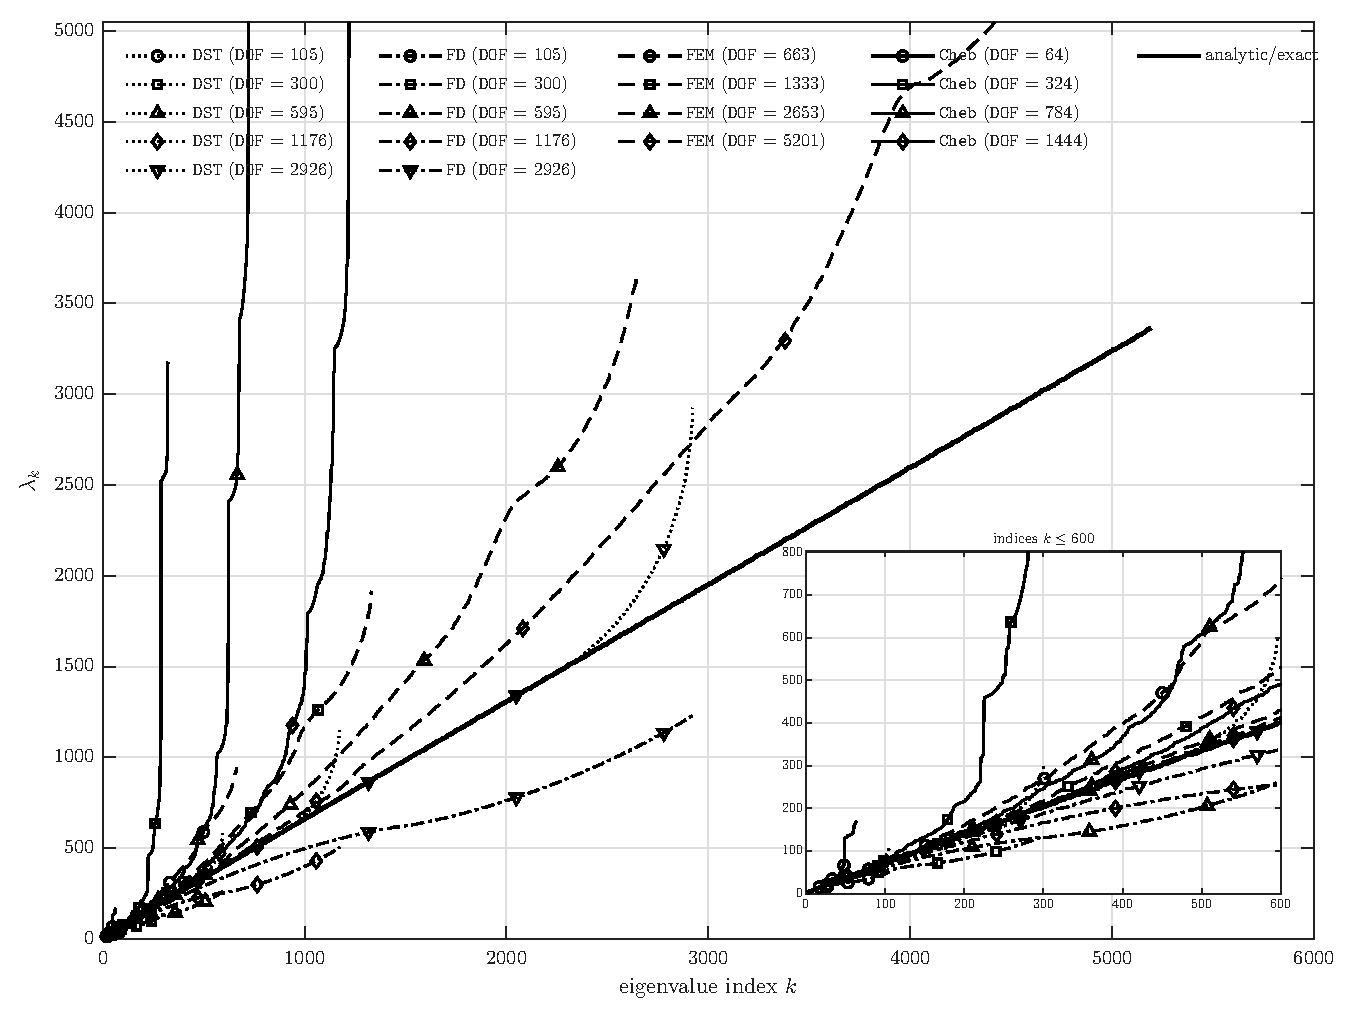
\includegraphics[width=0.85\textwidth]{rectangle_dof_sweep}}
  \\
  \subfloat[Right isosceles triangle, legs length~$\pi$.]{%
    
\includegraphics[width=0.85\textwidth]{isosceles_triangle_dof_sweep}}
  \caption{Eigenvalue DOF-sweep spectra.}
  \label{fig:dof_sweep}
\end{figure}

\begin{figure}[htbp]
  \centering
  
\includegraphics[width=0.85\textwidth]{L_shaped_dof_sweep}
  \caption{Eigenvalue DOF-sweep spectra for the L-shaped domain (square domain
    $2 \times 2$ minus a $1 \times 1$ top right corner).}
  \label{fig:dof_sweep_L_shaped}
\end{figure}
